\documentclass[12pt]{article}

\usepackage{bm}
\usepackage{amsmath, mathtools}
\usepackage{amsfonts}
\usepackage{amssymb}
\usepackage{graphicx}
\usepackage{colortbl}
\usepackage{xr}
\usepackage{hyperref}
\usepackage{longtable}
\usepackage{xfrac}
\usepackage{tabularx}
\usepackage{float}
\usepackage{siunitx}
\usepackage{booktabs}
\usepackage{caption}
\usepackage{pdflscape}
\usepackage{afterpage}

%\usepackage{refcheck}

\hypersetup{
    bookmarks=true,         % show bookmarks bar?
      colorlinks=true,       % false: boxed links; true: colored links
    linkcolor=red,          % color of internal links (change box color with linkbordercolor)
    citecolor=green,        % color of links to bibliography
    filecolor=magenta,      % color of file links
    urlcolor=cyan           % color of external links
}

%% Comments
\newif\ifcomments\commentstrue

\ifcomments
\newcommand{\authornote}[3]{\textcolor{#1}{[#3 ---#2]}}
\newcommand{\todo}[1]{\textcolor{red}{[TODO: #1]}}
\else
\newcommand{\authornote}[3]{}
\newcommand{\todo}[1]{}
\fi

\newcommand{\wss}[1]{\authornote{blue}{SS}{#1}}
\newcommand{\bmac}[1]{\authornote{red}{BM}{#1}}

\newcommand{\colZwidth}{1.0\textwidth}
\newcommand{\blt}{- } %used for bullets in a list
\newcommand{\colAwidth}{0.13\textwidth}
\newcommand{\colBwidth}{0.82\textwidth}
\newcommand{\colCwidth}{0.1\textwidth}
\newcommand{\colDwidth}{0.05\textwidth}
\newcommand{\colEwidth}{0.8\textwidth}
\newcommand{\colFwidth}{0.17\textwidth}
\newcommand{\colGwidth}{0.5\textwidth}
\newcommand{\colHwidth}{0.28\textwidth}
\newcounter{defnum} %Definition Number
\newcommand{\dthedefnum}{GD\thedefnum}
\newcommand{\dref}[1]{GD\ref{#1}}
\newcounter{datadefnum} %Datadefinition Number
\newcommand{\ddthedatadefnum}{DD\thedatadefnum}
\newcommand{\ddref}[1]{DD\ref{#1}}
\newcounter{theorynum} %Theory Number
\newcommand{\tthetheorynum}{T\thetheorynum}
\newcommand{\tref}[1]{T\ref{#1}}
\newcounter{tablenum} %Table Number
\newcommand{\tbthetablenum}{T\thetablenum}
\newcommand{\tbref}[1]{TB\ref{#1}}
\newcounter{assumpnum} %Assumption Number
\newcommand{\atheassumpnum}{P\theassumpnum}
\newcommand{\aref}[1]{A\ref{#1}}
\newcounter{goalnum} %Goal Number
\newcommand{\gthegoalnum}{P\thegoalnum}
\newcommand{\gsref}[1]{GS\ref{#1}}
\newcounter{instnum} %Instance Number
\newcommand{\itheinstnum}{IM\theinstnum}
\newcommand{\iref}[1]{IM\ref{#1}}
\newcounter{reqnum} %Requirement Number
\newcommand{\rthereqnum}{P\thereqnum}
\newcommand{\rref}[1]{R\ref{#1}}
\newcounter{lcnum} %Likely change number
\newcommand{\lthelcnum}{LC\thelcnum}
\newcommand{\lcref}[1]{LC\ref{#1}}

\newcommand{\tclad}{T_\text{CL}}
\newcommand{\degree}{\ensuremath{^\circ}}
\newcommand{\progname}{SWHS}

%\oddsidemargin 0mm
%\evensidemargin 0mm
%\textwidth 160mm
%\textheight 200mm
\usepackage{fullpage}

\begin{document}

\title{Software Requirements Specification for Solar Water Heating Systems
  Incorporating Phase Change Material} 
\author{Thulasi Jegatheesan, Brooks MacLachlan, and Spencer Smith}
\date{\today}
	
\maketitle

\tableofcontents

\section{Reference Material}

This section records information for easy reference.

\subsection{Table of Units}

Throughout this document SI (Syst\`{e}me International d'Unit\'{e}s) is employed
as the unit system.  In addition to the basic units, several derived units are
used as described below.  For each unit, the symbol is given followed by a
description of the unit and the SI name.
~\newline

\renewcommand{\arraystretch}{1.2}
%\begin{table}[ht]
  \noindent \begin{tabular}{l l l} 
    \toprule		
    \textbf{symbol} & \textbf{unit} & \textbf{SI}\\
    \midrule 
    \si{\metre} & length & metre\\
    \si{\kilogram} & mass	& kilogram\\
    \si{\second} & time & second\\
    \si{\celsius} & temperature & centigrade\\
    \si{\joule} & energy & Joule\\
    \si{\watt} & power & Watt (W = \si{\joule\per\second})\\
    \bottomrule
  \end{tabular}
  %	\caption{Provide a caption}
%\end{table}

\subsection{Table of Symbols}

The table that follows summarizes the symbols used in this document along with
their units.  The choice of symbols was made to be consistent with the heat
transfer literature and with existing documentation for solar water heating
systems.  The symbols are listed in alphabetical order.

\renewcommand{\arraystretch}{1.2}
%\noindent \begin{tabularx}{1.0\textwidth}{l l X}
\noindent \begin{longtable*}{l l p{12cm}} \toprule
  \textbf{symbol} & \textbf{unit} & \textbf{description}\\
  \midrule 
  $A_C$ & \si[per-mode=symbol] {\square\metre} & coil surface area
  \\
  $A_\text{in}$ & \si[per-mode=symbol] {\square\metre} & surface area over 
  which heat is transferred in
  \\ 
  $A_\text{out}$ & \si[per-mode=symbol] {\square\metre} & surface area over 
  which heat is transferred out
  \\
  $A_P$ & \si[per-mode=symbol] {\square\metre} & phase change material surface
  area
  \\ 
  $C$ & \si[per-mode=symbol] {\joule\per \kilogram\per \celsius} &
  specific heat capacity
  \\
  $C^L$ & \si[per-mode=symbol] {\joule\per\kilo\gram\per\celsius} & specific 
  heat capacity of a liquid 
  \\ 
  $C^L_P$ & \si[per-mode=symbol] {\joule\per \kilogram\per \celsius} & specific
  heat capacity of PCM as a liquid
  \\
  $C^S$ & \si[per-mode=symbol] {\joule\per\kilo\gram\per\celsius} & specific 
  heat capacity of a solid
  \\
  $C^S_P$ & \si[per-mode=symbol] {\joule\per \kilogram\per \celsius} & specific
  heat capacity of PCM as a solid
  \\
  $C^V$ & \si[per-mode=symbol] {\joule\per \kilogram\per \celsius} & specific
  heat capacity of a vapour
  \\
  $C_W$ & \si[per-mode=symbol] {\joule\per \kilogram\per \celsius} & specific
  heat capacity of water
  \\  
  $D$ & \si{\metre} & diameter of tank
  \\
  $E$ & \si[per-mode=symbol] {\joule} & sensible heat energy
  \\
  $E_{P\text{melt}}^\text{init}$ & \si[per-mode=symbol] {\joule} & heat energy
  in the PCM at the instant when melting begins
  \\ 
  $E_P$ & \si[per-mode=symbol] {\joule} & heat energy in the PCM
  \\ 
  $E_W$ & \si[per-mode=symbol] {\joule} & heat energy in the water
  \\ 
  $g$ & \si[per-mode=symbol] {\watt\per\cubic\metre} & volumetric heat
  generation per unit volume
  \\
  $h$ & \si[per-mode=symbol] {\watt\per\square\metre\per\celsius} & convective 
  heat transfer coefficient
  \\ 
  $h_C$ & \si[per-mode=symbol] {\watt\per\square\metre\per\celsius} &
  convective heat transfer coefficient between coil and water
  \\
  $H_f$ & \si[per-mode=symbol] {\joule \per \kilogram} & specific latent heat of
  fusion
  \\
  $h_P$ & \si[per-mode=symbol] {\watt\per\square\metre\per\celsius} &
  convective heat transfer coefficient between water and PCM
  \\
  $L$ & \si{\metre} & length of tank
  \\
  $m$ & \si[per-mode=symbol] {\kilo\gram} & mass
  \\
  $m_P$ & \si[per-mode=symbol] {\kilo\gram} & mass of phase change material
  \\
  $m_W$ & \si[per-mode=symbol] {\kilo\gram} & mass of water
  \\
  $\bf{\hat{n}}$ & \si[per-mode=symbol] {unitless} & unit outward normal 
  vector for a surface 
  \\ 
  $q$ & \si[per-mode=symbol] {\watt \per \square \metre} & heat
  flux
  \\
  $Q$ & \si[per-mode=symbol] {\joule} & latent heat energy
  \\
  $\bf{q}$ & \si[per-mode=symbol] {\watt\per\square\metre} & thermal flux vector
  \\
  $q_C$ & \si[per-mode=symbol] {\watt\per\square\metre} & heat flux from coil
  \\
  $q_\text{in}$ & \si[per-mode=symbol] {\watt\per\square\metre} & heat flux in
  \\ 
  $q_\text{out}$ & \si[per-mode=symbol] {\watt\per\square\metre} & heat flux out
  \\
  $q_P$ & \si[per-mode=symbol] {\watt\per\square\metre} & heat flux into phase
  change material
  \\
  $Q_P$ & \si[per-mode=symbol] {\joule} & latent heat energy added to PCM
  \\
  $R$ & unitless & Aspect ratio (ratio of tank diameter ($D$) to tank length
  ($L$) %CHANGE
  \\ 
  $S$ & \si[per-mode=symbol] {unitless} & surface
  \\
  $t$ & \si[per-mode=symbol] {\second} & time
  \\
  $T$ & \si[per-mode=symbol] {\celsius} & temperature
  \\
  $T_\text{boil}$ & \si[per-mode=symbol] {\celsius} & temperature at boiling point
  \\
  $T_C$ &\si[per-mode=symbol] {\celsius} & temperature of coil
  \\
  $T_\text{env}$ & \si[per-mode=symbol] {\celsius} & temperature of environment
  \\ 
  $t_\text{final}$ & \si[per-mode=symbol] {\second} & final time
  \\ 
  $T_\text{init}$ & \si[per-mode=symbol] {\celsius} & initial temperature
  \\
  $T_\text{melt}$ & \si[per-mode=symbol] {\celsius} & temperature at melting point
  \\
  $t_\text{melt}^\text{init}$ & \si[per-mode=symbol] {\second} & time at which
                                                                 melting of PCM begins
  \\ 
  $t_\text{melt}^\text{final}$ & \si[per-mode=symbol] {\second} & time at which
                                                                 melting of PCM ends
  \\ 
  $T_\text{melt}^{P}$ & \si[per-mode=symbol] {\celsius} & temperature at melting
                                                          point for PCM
  \\
  $T_P$ & \si[per-mode=symbol] {\celsius} & temperature of phase change material
  \\
  $T_W$ & \si[per-mode=symbol] {\celsius} & temperature of water
  \\
  $V$ & \si[per-mode=symbol] {\cubic\metre} & volume
  \\
  $V_P$ & \si[per-mode=symbol] {\cubic\metre} & volume of PCM
  \\
  $V_\text{tank}$ & \si[per-mode=symbol] {\cubic\metre} & volume of the
  cylindrical tank
  \\
  $V_W$ & \si[per-mode=symbol] {\cubic\metre} & volume of water
  \\
  $\Delta T$ & \si[per-mode=symbol] {\celsius} & temperature difference
  \\
  $\eta$ & \si[per-mode=symbol] {unitless} & ODE parameter
  \\
  $\rho$ & \si[per-mode=symbol] {\kilogram\per\cubic\metre} & density, mass per
  unit volume
  \\
  $\rho_P$ & \si[per-mode=symbol] {\kilogram\per\cubic\metre} & density of PCM
  \\
  $\rho_W$ & \si[per-mode=symbol] {\kilogram\per\cubic\metre} & density of water
  \\
  $\tau$ & \si[per-mode=symbol] {\second} & dummy variable for integration over time
  \\
  $\tau_P^L$ & \si[per-mode=symbol] {\second} & ODE parameter for liquid PCM
  \\
  $\tau_P^S$ & \si[per-mode=symbol] {\second} & ODE parameter for solid PCM
  \\
  $\tau_W$ & \si[per-mode=symbol] {\second} & ODE parameter for water
  \\
  $\phi$ & \si[per-mode=symbol] {unitless} & melt fraction
  \\
  \bottomrule
\end{longtable*}

%\noindent \textbf{Prefixes}\\
%~\newline

%\noindent
%\begin{tabular}{l l}
%$\Delta$ & \blt finite change in following quantity\\
%$d$ & \blt infinitesimal change in the following quantity\\
%\end{tabular}\\
%~\newline

\subsection{Abbreviations and Acronyms}

\renewcommand{\arraystretch}{1.2}
\begin{tabular}{l l} 
  \toprule		
  \textbf{symbol} & \textbf{description}\\
  \midrule 
  A & Assumption\\
  DD & Data Definition\\
  GD & General Definition\\
  GS & Goal Statement\\
  IM & Instance Model\\
  LC & Likely Change\\
  ODE & Ordinary Differential Equation\\
  PCM & Phase Change Material\\
  PS & Physical System Description\\
  R & Requirement\\
  RHS & Right Hand Side\\
  SRS & Software Requirements Specification\\
  \progname{} & Solar Water Heating System\\
  T & Theoretical Model\\
  \bottomrule
\end{tabular}\\

\section{Introduction}

Due to the increasing cost, diminishing availability, and negative environmental
impact of fossil fuels, there is a higher demand for renewable energy sources
and energy storage technology.  Solar water heating systems incorporating Phase
Change Material (PCM) use a renewable energy source and provide a novel way of
storing energy.  Solar water heating systems with PCM improve over the
traditional solar heating systems because of their smaller size.  The smaller
size is possible because of the ability of PCM to store thermal energy as latent
heat, which allows higher thermal energy storage capacity per unit weight.

The following section provides an overview of the Software Requirements
Specification (SRS) for a solar water heating system that incorporates PCM.  The
developed program will be referred to as Solar Water Heating System
(\progname{}).  This section explains the purpose of this document, the scope of
the system, the characteristics of the intended readers and the organization of
the document.

\subsection{Purpose of Document}

The main purpose of this document is to describe the modelling of solar water
heating systems incorporating PCM.  The goals and theoretical models used in the 
\progname{} code are provided, with an emphasis on explicitly identifying 
assumptions and unambiguous definitions.  This document is intended to be used 
as a reference to provide ad hoc access to all information necessary to 
understand and verify the model.  The SRS is abstract because the contents say
\emph{what} problem is being solved, but do not say \emph{how} to solve it.

This document will be used as a starting point for subsequent development
phases, including writing the design specification and the software verification
and validation plan.  The design document will show how the requirements are to
be realized, including decisions on the numerical algorithms and programming
environment.  The verification and validation plan will show the steps that will
be used to increase confidence in the software documentation and the
implementation.  Although the SRS fits in a series of documents that follow the
so-called waterfall model, the actual development process is not constrained in
any way.  Even when the process is not waterfall, as Parnas and
Clements~\cite{ParnasAndClements1986} point out, the most logical way to present
the documentation is still to ``fake'' a rational design process.

\subsection{Scope of Requirements} 

The scope of the requirements is limited to thermal analysis of a single solar
water heating tank incorporating PCM.  Given the appropriate inputs, the code
for \progname{} is intended to predict the temperature and energy histories for
the water and the PCM.  This entire document is written assuming that the
substances inside the heating tank are water and PCM.

\subsection{Characteristics of Intended Reader} 

Reviewers of this documentation should have a strong knowledge in heat transfer
theory.  A third or fourth year Mechanical Engineering course on this topic is
recommended.  The reviewers should also have an understanding of differential
equations, as typically covered in first and second year Calculus courses.  The
users of \progname{} can have a lower level of expertise, as explained in
Section~\ref{SecUserCharacteristics}.

\subsection{Organization of Document}

The organization of this document follows the template for an SRS for scientific
computing software proposed by~\cite{Koothoor2013} and \cite{SmithAndLai2005}.
The presentation follows the standard pattern of presenting goals, theories,
definitions, and assumptions.  For readers that would like a more bottom up
approach, they can start reading the instance models in Section
\ref{sec_instance} and trace back to find any additional information they
require.  The instance models provide the Ordinary Differential Equations (ODEs)
and algebraic equations that model the solar water heating system with PCM.
\progname{} solves these ODEs.

The goal statements are refined to the theoretical models, and theoretical
models to the instance models.  The instance models (Section \ref{sec_instance})
to be solved are referred to as \iref{ewat} to \iref{I_HPCM}.

\section{General System Description}

This section identifies the interfaces between the system and its environment,
describes the user characteristics and lists the system constraints.

\subsection{System Context}

Figure~\ref{Fig_SystemContext} shows the system context.  A circle represents an
external entity outside the software, the user in this case.  A rectangle
represents the software system itself (\progname{}).  Arrows are used to show the data
flow between the system and its environment.

\begin{figure}[h!]
\begin{center}
 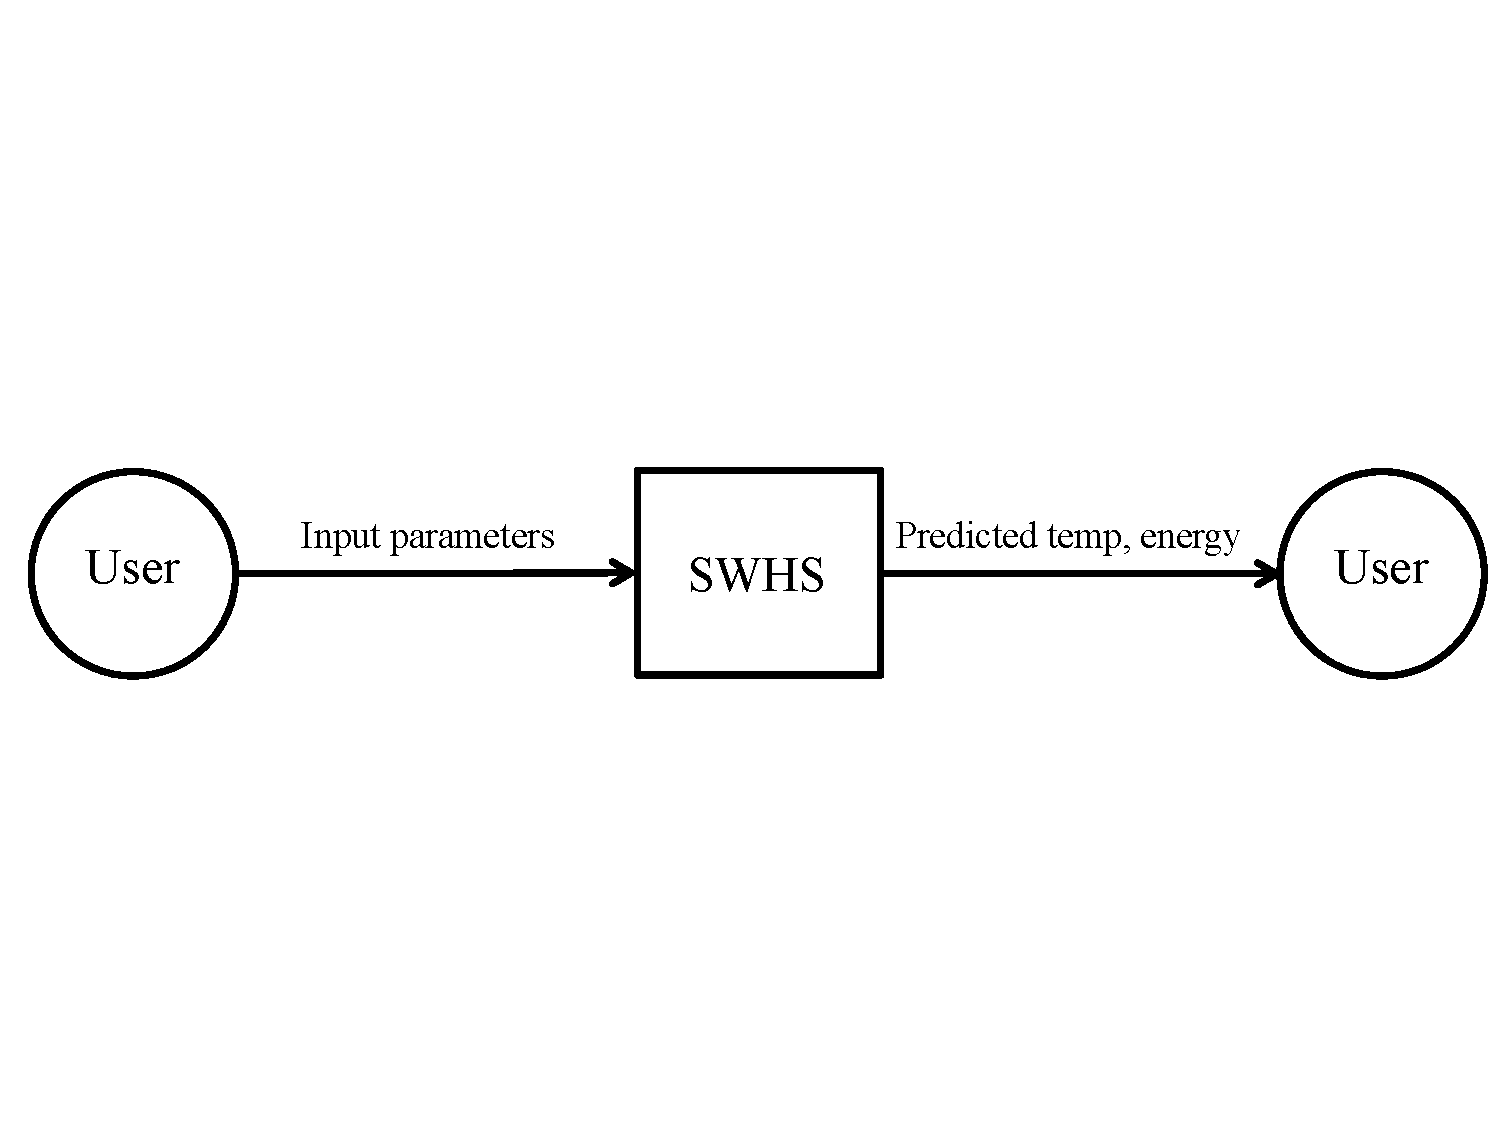
\includegraphics[width=0.6\textwidth]{SystemContextFigure}
\caption{System Context}
\label{Fig_SystemContext} 
\end{center}
\end{figure}

\progname{} is mostly self-contained.  The only external interaction is through
the user interface.  The responsibilities of the user and the system are as
follows:

\begin{itemize}
\item User Responsibilities:
\begin{itemize}
\item Provide the input data to the system, ensuring no errors in the data entry
\item Take care that consistent units are used for input variables
\end{itemize}
\item \progname{} Responsibilities:
\begin{itemize}
\item Detect data type mismatch, such as a string of characters instead of a
  floating point number
\item Determine if the inputs satisfy the required physical and software constraints
\item Calculate the required outputs
\end{itemize}
\end{itemize}

\subsection{User Characteristics} \label{SecUserCharacteristics}

The end user of \progname{} should have an understanding of undergraduate Level
1 Calculus and Physics.

\subsection{System Constraints}

There are no system constraints.

\section{Specific System Description}

This section first presents the problem description, which gives a high-level
view of the problem to be solved.  This is followed by the solution characteristics
specification, which presents the assumptions, theories, definitions and finally
the instance models (ODEs) that model the solar water heating tank with PCM.

\subsection{Problem Description} \label{Sec_pd}

\progname{} is a computer program developed to investigate the effect of
employing PCM within a solar water heating tank.

%\subsubsection{Background}

\subsubsection{Terminology and  Definitions}

This subsection provides a list of terms that are used in the subsequent
sections and their meaning, with the purpose of reducing ambiguity and making it
easier to correctly understand the requirements:

\begin{itemize}

\item Heat Flux: The rate of heat energy transfer per unit area.

\item Phase Change Material (PCM): A substance that uses phase changes (such as melting)
  to absorb or release large amounts of heat at a constant temperature.

\item Specific Heat: heat capacity per unit mass.

\item Thermal Conduction: the transfer of heat energy through a substance.

\item Transient: Changing with time.

\end{itemize}

\subsubsection{Physical System Description}

The physical system of \progname{}, as shown in Figure~\ref{Fig_Tank},
includes the following elements:

\begin{itemize}

\item[PS1:] Tank containing water.

\item[PS2:] Heating coil at bottom of tank.  ($q_C$ represents the heat flux
  from the coil into the water.)

\item[PS3:] PCM suspended in tank.  ($q_P$ represents
  the heat flux from the water into the PCM.)

\end{itemize}

\begin{figure}[h!]
\begin{center}
%\rotatebox{-90}
{
 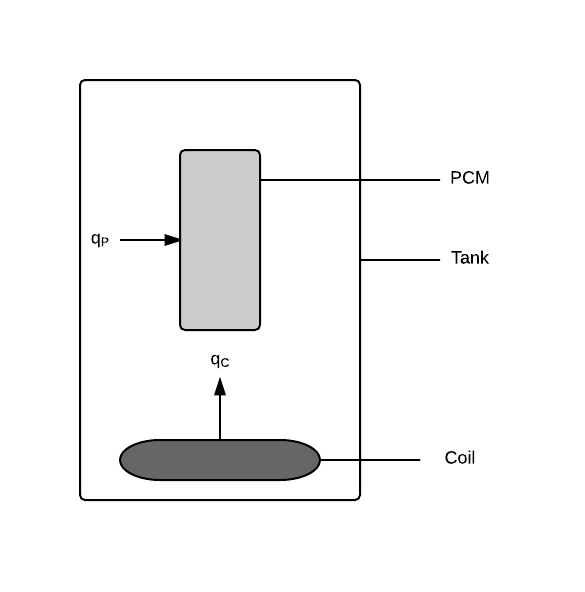
\includegraphics[width=0.5\textwidth]{Tank.png}
}
\caption{\label{Fig_Tank} Solar water heating tank, with heat flux from coil 
and to the PCM of $q_C$ and $q_P$, respectively}
\end{center}
\end{figure}

\subsubsection{Goal Statements}

\noindent Given the temperature of the coil, initial conditions for the temperature of 
the water and the PCM, and material properties, the goal statements are:

\begin{itemize}

\item[GS\refstepcounter{goalnum}\thegoalnum \label{G_wtemp}:] Predict the water 
temperature over time.

\item[GS\refstepcounter{goalnum}\thegoalnum \label{G_ptemp}:] Predict the PCM 
temperature over time.
	
\item[GS\refstepcounter{goalnum}\thegoalnum \label{G_wenergy}:] Predict the 
change in the energy of the water over time.

\item[GS\refstepcounter{goalnum}\thegoalnum \label{G_penergy}:] Predict the 
change in the energy of the PCM over time.

\end{itemize}

\subsection{Solution Characteristics Specification}

The instance models (ODEs) that govern \progname{} are presented in
Subsection~\ref{sec_instance}.  The information to understand the meaning of the
instance models and their derivation is also presented, so that the instance
models can be verified.

\subsubsection{Assumptions}

This section simplifies the original problem and helps in developing the
theoretical model by filling in the missing information for the physical
system. The numbers given in the square brackets refer to the theoretical model
[T], general definition [GD], data definition [DD], instance model [IM], or
likely change [LC], in which the respective assumption is used.

\begin{itemize}

\item[A\refstepcounter{assumpnum}\theassumpnum \label{A_OnlyThermalEnergy}:] The
  only form of energy that is relevant for this problem is thermal energy.  All
  other forms of energy, such as mechanical energy, are assumed to be
  negligible [\tref{T_COE}].

\item[A\refstepcounter{assumpnum}\theassumpnum \label{A_hcoeff}:] All heat
  transfer coefficients are constant over time [\dref{NL}].

\item[A\refstepcounter{assumpnum}\theassumpnum \label{A_mixed}:] The water in
  the tank is fully mixed, so the temperature is the same throughout the entire
  tank [\dref{ROCT}, \ddref{FluxPCM}].

\item[A\refstepcounter{assumpnum}\theassumpnum \label{A_tpcm}:] The PCM has the
  same temperature throughout [\dref{ROCT}, \ddref{FluxPCM}, \lcref{LC_tpcm}].

\item[A\refstepcounter{assumpnum}\theassumpnum \label{A_const_density}:] Density
  of the water and PCM have no spatial variation; that is, they are each
  constant over their entire volume [\dref{ROCT}].

\item[A\refstepcounter{assumpnum}\theassumpnum \label{A_const_C}:] Specific heat
  capacity of the water and PCM have no spatial variation; that is, they are
  each constant over their entire volume [\dref{ROCT}].

\item[A\refstepcounter{assumpnum}\theassumpnum \label{A_Newt_coil}:] Newton's
  law of convective cooling applies between the coil and the water [\ddref{FluxCoil}].
	
\item[A\refstepcounter{assumpnum}\theassumpnum \label{A_tcoil}:] The temperature
  of the heating coil is constant over time [\ddref{FluxCoil}, \lcref{LC_tcoil}].
	
\item[A\refstepcounter{assumpnum}\theassumpnum \label{A_tlcoil}:] The
  temperature of the heating coil does not vary along its
  length [\ddref{FluxCoil}, \lcref{LC_tlcoil}].

\item[A\refstepcounter{assumpnum}\theassumpnum \label{A_Newt_pcm}:] Newton's law
  of convective cooling applies between the water and the PCM [\ddref{FluxPCM}].

\item[A\refstepcounter{assumpnum}\theassumpnum \label{A_charge}:] The model only
  accounts for charging of the tank, not discharging.  The temperature of the
  water and PCM can only increase, or remain constant; they do not decrease.
  This implies that the initial temperature (\aref{A_InitTemp}) is less than (or
  equal) to the temperature of the coil [\iref{ewat}, \lcref{LC_charge}].

\item[A\refstepcounter{assumpnum}\theassumpnum \label{A_InitTemp}:] The
  initial temperature of the water and the PCM is the same [\iref{ewat},
  \iref{epcm}, \lcref{LC_InitTemp}].

\item[A\refstepcounter{assumpnum}\theassumpnum \label{A_OpRangePCM}:] The
  simulation will start with the PCM in solid form [\iref{epcm}, \iref{I_HPCM}].

\item[A\refstepcounter{assumpnum}\theassumpnum \label{A_OpRange}:] The operating
  temperature range of the system is such that the water is always in liquid
  form.  That is, the temperature will not drop below the melting point of water, or rise
  above its boiling point [\iref{ewat}, \iref{I_HWAT}].

\item[A\refstepcounter{assumpnum}\theassumpnum \label{A_htank}:] The tank is
  perfectly insulated so that there is no heat loss from the tank [\iref{ewat},
  \lcref{LC_htank}].

\item[A\refstepcounter{assumpnum}\theassumpnum \label{A_int_heat}:] No internal
  heat is generated by either the water or the PCM; therefore, the volumetric
  heat generation is zero [\iref{ewat}, \iref{epcm}].
	
\item[A\refstepcounter{assumpnum}\theassumpnum \label{A_vpcm}:] The volume
  change of the PCM due to melting is negligible [\iref{epcm}].

\item[A\refstepcounter{assumpnum}\theassumpnum \label{A_PCM_state}:] The PCM is
  either in a liquid or solid state, but not a gas [\iref{epcm}, \iref{I_HPCM}].
  
\item[A\refstepcounter{assumpnum}\theassumpnum \label{A_Pressure}:] The pressure
  in the tank is atmospheric, so the melting and boiling points of water are
  $0^o\text{C}$ and $100^o\text{C}$, respectively [\iref{ewat}, \iref{I_HWAT}].

\item[A\refstepcounter{assumpnum}\theassumpnum \label{A_VolCoil}:] When
  considering the volume of water in the tank, the volume of the coil is assumed
  to be negligible [\rref{R_MassInputs}].
	
\end{itemize}

\subsubsection{Theoretical Models}\label{sec_theoretical}

This section focuses on the general equations and laws that \progname{} is based
on.

~\newline

\noindent
\begin{minipage}{\textwidth}
\renewcommand*{\arraystretch}{1.5}
\begin{tabular}{| p{\colAwidth} | p{\colBwidth}|}
  \hline
  \rowcolor[gray]{0.9}
  Number& T\refstepcounter{theorynum}\thetheorynum \label{T_COE}\\
  \hline
  Label&\bf Conservation of thermal energy\\
  \hline
  Equation&  $-{\bf \nabla \cdot q} + g$ = $\rho C \frac{\partial T}{\partial t}$\\
  \hline
  Description & 
  The above equation gives the conservation of energy for transient heat transfer in a material
  of specific heat capacity $C$ (\si{\joule\per\kilogram\per\celsius}) and density $\rho$ 
  (\si{\kilogram\per\cubic\metre}), where $\bf q$ is the thermal flux vector (\si{\watt\per\square\metre}),
  $g$ is the volumetric heat generation (\si{\watt\per\cubic\metre}), $T$ is the temperature (\si{\celsius}), $t$ is time (\si{\second}), and $\nabla$ is the gradient operator.  For this equation to apply, other forms of energy, such as mechanical energy, are assumed to be negligible in the
  system (\aref{A_OnlyThermalEnergy}).  In general, the material properties ($\rho$ and $C$) depend on temperature.\\
  \hline
  Source &
  \url{http://www.efunda.com/formulae/heat_transfer/conduction/overview_cond.cfm}\\
  % The above web link should be replaced with a proper citation to a publication
  \hline
  Ref.\ By & \dref{ROCT}\\
  \hline
\end{tabular}
\end{minipage}\\

~\newline

\noindent
\begin{minipage}{\textwidth}
\renewcommand*{\arraystretch}{1.5}
\begin{tabular}{| p{\colAwidth} | p{\colBwidth}|}
  \hline
  \rowcolor[gray]{0.9}
  Number& T\refstepcounter{theorynum}\thetheorynum \label{T_SHE}\\
  \hline
  Label&\bf Sensible heat energy\\
  \hline
  Equation&  
  $
  E = \begin{cases}
  C^{S}m\Delta T & \text { if } T < T_\text{melt}\\
  C^{L}m\Delta T & \text { if }  T_\text{melt}<T < T_\text{boil}\\
  C^{V}m\Delta T & \text { if }  T_\text{boil}<T \\
  \end{cases}
  $
  \\
  &See \tref{T_LHE}, Latent heat energy, if $T$ = $T_\text{boil}$ or 
  $T$ = $T_\text{melt}$.\\
  
  \hline
  Description & $E$ is the change in sensible heat energy (\si{\joule}).\\
  & $C^S$, $C^L$, $C^V$ are the specific heat capacities of a solid, liquid, 
	and vapour, respectively (\si{\joule\per\kilogram\per\celsius}).\\
  & $m$ is the mass (\si{\kilogram}).\\
  & $T$ is the temperature (\si{\celsius}), and $\Delta T$ is the change in temperature (\si{\celsius}).\\
  & $T_\text{melt}$ and $T_\text{boil}$ are the melting and boiling points, respectively (\si{\celsius}).\\
  & Sensible heating occurs as long as the material does not reach a temperature 
  where a phase change occurs.\\
  & A phase change occurs if $T = T_\text{boil}$ or $T = T_\text{melt}$.  
  If this is the case, refer to \tref{T_LHE}, Latent heat energy.
  \\
  \hline
  Source &
  \url{http://en.wikipedia.org/wiki/Sensible_heat}\\
  % The above web link should be replaced with a proper citation to a publication
  \hline
  Ref.\ By & \iref{I_HWAT}, \iref{I_HPCM}\\
  \hline
\end{tabular}
\end{minipage}\\

%\wss{Please add units for the variables without them.}

~\newline

\noindent
\begin{minipage}{\textwidth}
\renewcommand*{\arraystretch}{1.5}
\begin{tabular}{| p{\colAwidth} | p{\colBwidth}|}
  \hline
  \rowcolor[gray]{0.9}
  Number& T\refstepcounter{theorynum}\thetheorynum \label{T_LHE}\\
  \hline
  Label&\bf Latent heat energy\\
  \hline
  Equation& $T=T_\text{melt}$ or $T = T_\text{boil}$, $Q(t)$ = 
  $\int_0^t \frac{dQ(\tau)}{d\tau}d\tau$, with $Q(0)=0$\\
  \hline
  Description & $Q$ is the change in thermal energy (\si{\joule}), latent heat energy.\\
  &$\int_0^t \frac{dQ(\tau)}{d\tau}d\tau$ is the rate of change of $Q$ with respect 
  to time $\tau$ (\si{\second}).  $t$ is the time (\si{\second}) elapsed, as long as the phase change is not complete.
  The status of the phase change depends on the melt fraction \ddref{D_MF}.\\
  & $T_\text{melt}$ and $T_\text{boil}$ are the melting and boiling points, respectively (\si{\celsius}).\\
  & Latent heating stops when all material has changed to the new phase. 
  \\
  \hline
  Source &
  \url{http://en.wikipedia.org/wiki/Latent_heat}\\
  % The above web link should be replaced with a proper citation to a publication
  \hline
  Ref.\ By & \tref{T_SHE}, \iref{I_HPCM}\\
  \hline
\end{tabular}
\end{minipage}\\

%\wss{The quantities $T_\text{melt}$ of $T_\text{boil}$ should be mentioned in
%  the description.}

%~\newline

\subsubsection{General Definitions}\label{sec_gendef}

This section collects  the laws and equations that will be used in deriving the
data definitions, which in turn are used to  build the instance models.

~\newline

\noindent
\begin{minipage}{\textwidth}
\renewcommand*{\arraystretch}{1.5}
\begin{tabular}{| p{\colAwidth} | p{\colBwidth}|}
\hline
\rowcolor[gray]{0.9}
Number& GD\refstepcounter{defnum}\thedefnum \label{NL}\\
\hline
Label &\bf Newton's law of cooling \\
\hline
% Units&$MLt^{-3}T^0$\\
% \hline
SI Units&\si{\watt\per\square\metre}\\
\hline
Equation&$ q(t) = h \Delta T(t)$  \\
\hline
Description &
Newton's law of cooling describes convective cooling from a surface.  The law is
stated as: the rate of heat loss from a body is proportional to the difference
in temperatures between the body and its surroundings.
\\
& $q(t)$ is the thermal flux (\si{\watt\per\square\metre}).\\
& $h$ is the heat transfer coefficient, assumed independent of $T$ (\aref{A_hcoeff})
	(\si{\watt\per\square\metre\per\celsius}).\\
&$\Delta T(t)$= $T(t) - T_{\text{env}}(t)$ is the time-dependent thermal gradient
between the environment and the object (\si{\celsius}).
\\
\hline
  Source &~\cite[p.\ 8]{Incropera2007}\\
  \hline
  Ref.\ By & \ddref{FluxCoil}, \ddref{FluxPCM}\\
  \hline
\end{tabular}
\end{minipage}\\

~\newline

\noindent
\begin{minipage}{\textwidth}
\renewcommand*{\arraystretch}{1.5}
\begin{tabular}{| p{\colAwidth} | p{\colBwidth}|}
  \hline
  \rowcolor[gray]{0.9}
  Number& GD\refstepcounter{defnum}\thedefnum \label{ROCT}\\
  \hline
  Label &\bf Simplified rate of change of temperature \\
  \hline
  Equation&$m C \frac{dT}{dt} = q_{\mathrm{in}} A_{\mathrm{in}} - 
  q_{\mathrm{out}} A_{\mathrm{out}} + g V$  \\
  \hline
  Description & The basic equation governing the rate of change of temperature,
  for a given volume $V$, with time.\\
  &$m$ is the mass (kg).\\
  &$C$ is the specific heat capacity (\si{\joule \per\kilogram \per\celsius}).\\
  & $T$ is the temperature (\si{\celsius}) and $t$ is the time (\si{\second}).\\
  & $q_{\mathrm{in}}$ and $q_{\mathrm{out}}$ are the in and out heat transfer
  rates, respectively (\si{\watt\per\square\metre}).\\
  & $A_{\mathrm{in}}$ and $A_{\mathrm{out}}$ are the surface areas over which the 
  heat is being transferred in and out, respectively (\si{\square\metre}).\\
  &$g$ is the volumetric heat generated (\si{\watt\per\cubic\metre}).\\
  &$V$ is the volume (\si{\cubic\metre}).
  \\
  \hline
  Ref.\ By & \iref{ewat}, \iref{epcm}\\
  \hline
\end{tabular}
\end{minipage}\\

\subsubsection*{Detailed derivation of simplified rate of change of temperature}

Integrating (\tref{T_COE}) over a volume ($V$), we have

\begin{equation*}
-\int_V{\bf \nabla q} dV+\int_V g dV= \int_V \rho C \frac{\partial T}{\partial t}dV.
\end{equation*}

\noindent
Applying Gauss's Divergence theorem to the first term over the surface $S$ of
the volume, with
\textbf{q} as the thermal flux vector for the surface, and {$\mathbf{\hat n}$} as
a unit outward normal for the surface,

\begin{equation}
-\int_S{ \bf{q\cdot \hat n}} dS+\int_V g dV= \int_V \rho C \frac{\partial T}{\partial t}dV. \label{eq:1}
\end{equation}

\noindent
We consider an arbitrary volume.  The volumetric heat generation is assumed
constant.  Then (\ref{eq:1}) can be written as

%If the heat flux over the surface that adds energy can be written as
% $q_{\mathrm{in}}$, while the heat flux leaving the body can be written as
% $q_{\mathrm{out}}$, (\ref{eq:1}) can be written as

\begin{equation*}
  q_{\mathrm{in}} A_{\mathrm{in}} - q_{\mathrm{out}} A_{\mathrm{out}} + g V = \int_V \rho C \frac{\partial T}{\partial t}dV,
\end{equation*}

\noindent where $q_{\mathrm{in}}$, $q_{\mathrm{out}}$, $A_{\mathrm{in}}$, and 
$A_{\mathrm{out}}$ are explained in \dref{ROCT}.  Assuming $\rho$, $C$ and $T$ are
constant over the volume, which is true in our case by assumptions (\aref{A_mixed}),
(\aref{A_tpcm}), (\aref{A_const_density}), and (\aref{A_const_C}), we have

\begin{equation}
\rho C V\frac{dT}{dt} = q_{\mathrm{in}} A_{\mathrm{in}} - q_{\mathrm{out}} A_{\mathrm{out}} + g V. \label{eq:2}
\end{equation}

\noindent
Using the fact that $\rho = {m}/{V}$, (\ref{eq:2}) can be written as

\begin{equation*}
m C \frac{dT}{dt} = q_{\mathrm{in}} A_{\mathrm{in}} - q_{\mathrm{out}} A_{\mathrm{out}} + g V.
\end{equation*}

\subsubsection{Data Definitions}\label{sec_datadef}

This section collects and defines all the data needed to build the instance
models. The dimension of each quantity is also given.

~\newline

\noindent
\begin{minipage}{\textwidth}
\renewcommand*{\arraystretch}{1.5}
\begin{tabular}{| p{\colAwidth} | p{\colBwidth}|}
\hline
\rowcolor[gray]{0.9}
Number& DD\refstepcounter{datadefnum}\thedatadefnum \label{FluxCoil}\\
\hline
Label& \bf Heat flux out of coil\\
\hline
Symbol &$q_C$\\
\hline
% Units& $Mt^{-3}$\\
% \hline
SI Units & \si{\watt\per\square\metre}\\
\hline
Equation&$q_C(t) = h_C (T_C - T_W(t))$, over area $A_C$\\
\hline
Description & 
$T_C$ is the temperature of the coil (\si{\celsius}).  $T_W$ is the temperature of the water (\si{\celsius}).  
The heat flux out of the coil, $q_C$ (\si{\watt\per\square\metre}), is found by assuming that Newton's Law of Cooling applies (\aref{A_Newt_coil}).  This law (\dref{NL}) is used on the surface of
the coil, which has area $A_C$ (\si{\square\metre}) and heat 
transfer coefficient $h_C$ (\si{\watt\per\square\metre\per\celsius}).  This equation assumes that the temperature of the coil is constant over time (\aref{A_tcoil}) and that it does not vary along the length
of the coil (\aref{A_tlcoil}).
\\
\hline
Sources&~\cite{Lightstone2012}  \\
\hline
Ref.\ By & \iref{ewat}\\
\hline
\end{tabular}
\end{minipage}\\

~\newline

%\wss{It would be nice for this data definition, and all of the other ones, to
%  have units listed for quantities after their first appearance.}

\noindent
\begin{minipage}{\textwidth}
\renewcommand*{\arraystretch}{1.5}
\begin{tabular}{| p{\colAwidth} | p{\colBwidth}|}
\hline
\rowcolor[gray]{0.9}
Number& DD\refstepcounter{datadefnum}\thedatadefnum \label{FluxPCM}\\
\hline
Label& \bf Heat flux into PCM\\
\hline
Symbol &$q_P$\\
\hline
% Units&$Mt^{-3}$\\
% \hline
SI Units & \si{\watt\per\square\metre}\\
\hline
Equation&$q_P(t) = h_P (T_W(t) - T_P(t))$, over area $A_P$\\
\hline
Description & 
$T_W$ is the temperature of the water (\si{\celsius}).  $T_P$ is the temperature of the PCM (\si{\celsius}).  
The heat flux into the PCM, $q_P$ (\si{\watt\per\square\metre}), is found by assuming that Newton's Law of Cooling applies (\aref{A_Newt_pcm}).  This law (\dref{NL}) is used on the surface of the PCM, which has area $A_P$ (\si{\square\metre}) and heat transfer coefficient $h_P$ (\si{\watt\per\square\metre\per\celsius}).    This equation assumes that the temperature of the PCM and water each have constant values over the surface area over which they interact
(\aref{A_mixed} and \aref{A_tpcm}).
\\
\hline
Sources&~\cite{Lightstone2012}  \\
\hline
Ref.\ By & \iref{ewat}, \iref{epcm}, \iref{I_HPCM}\\
\hline
\end{tabular}
\end{minipage}\\


% ~\newline

% \noindent
% \begin{minipage}{\textwidth}
% \renewcommand*{\arraystretch}{1.5}
% \begin{tabular}{| p{\colAwidth} | p{\colBwidth}|}
% \hline
% \rowcolor[gray]{0.9}
% Number& DD\refstepcounter{datadefnum}\thedatadefnum \label{BalanceConstant1}\\
% \hline
% Label& \bf Energy Balance Constant 1\\
% \hline
% Symbol &$\tau_W$\\
% \hline
% Units&$t^2$\\
% \hline
% SI Units &$\mathrm{\frac{J}{W}}$\\
% \hline
% Equation&$\tau_W = \frac{m_W C_W}{h_C A_C}$\\
% \hline
% Description & 
% $\tau_W$ is a constant comprised of the mass of the water $m_W$,
% the specific heat capacity of water $C_W$, the heat transfer 
% coefficient of the coil $h_C$, and the surface area of the coil, $A_C$.
% \\
% \hline
 % Sources&  \\
% \hline
% \end{tabular}
% \end{minipage}\\

% ~\newline

% \noindent
% \begin{minipage}{\textwidth}
% \renewcommand*{\arraystretch}{1.5}
% \begin{tabular}{| p{\colAwidth} | p{\colBwidth}|}
% \hline
% \rowcolor[gray]{0.9}
% Number& DD\refstepcounter{datadefnum}\thedatadefnum \label{BalanceConstant2}\\
% \hline
% Label& \bf Energy Balance Constant 2\\
% \hline
% Symbol &$\eta$\\
% \hline
% Units& dimensionless\\
% \hline
% SI Units & dimensionless\\
% \hline
% Equation&$\eta = \frac{h_P A_P}{h_C A_C}$\\
% \hline
% Description & 
% $\eta$ is a constant comprised of the heat transfer coefficient of the PCM ($h_P$), 
% the surface area of the PCM ($A_P$), the heat transfer coefficient of the coil ($h_C$), 
% and the surface area of the coil ($A_C$).
% \\
% \hline
 % Sources&  \\
% \hline
% \end{tabular}
% \end{minipage}\\

% ~\newline

% \noindent
% \begin{minipage}{\textwidth}
% \renewcommand*{\arraystretch}{1.5}
% \begin{tabular}{| p{\colAwidth} | p{\colBwidth}|}
% \hline
% \rowcolor[gray]{0.9}
% Number& DD\refstepcounter{datadefnum}\thedatadefnum \label{BalanceConstant3}\\
% \hline
% Label& \bf Energy Balance Constant 3\\
% \hline
% Symbol &$\tau_P$\\
% \hline
% Units& $T t^3 L^{-2}$\\
% \hline
% SI Units &$\frac{{\mathrm{kg}}{\mathrm{^oC}}}{\mathrm{W}}$\\
% \hline
% Equation&$\tau_P = \frac{m_P}{h_P A_P}$\\
% \hline
% Description & 
% $\tau_P$ is a constant comprised of the mass of the PCM ($m_P$), the heat transfer 
% coefficient of the PCM ($h_P$), and the surface area of the PCM ($A_P$).
% \\
% \hline
 % Sources&  \\
% \hline
% \end{tabular}
% \end{minipage}\\

~\newline

\noindent
\begin{minipage}{\textwidth}
\renewcommand*{\arraystretch}{1.5}
\begin{tabular}{| p{\colAwidth} | p{\colBwidth}|}
  \hline
  \rowcolor[gray]{0.9}
  Number& DD\refstepcounter{datadefnum}\thedatadefnum \label{D_HOF}\\
  \hline
  Label& \bf Specific latent heat of fusion\\
  \hline
  Symbol &$H_f$\\
  \hline
  % Units&$M^2 L^2 t^{-2}$\\
  % \hline
  SI Units &$\si{\joule \per \kilogram}$\\
  \hline
  Equation&$H_f$ = $\frac{Q}{m}$\\
  \hline
  Description & 
  $H_f$ is the amount of heat energy required to completely melt a unit mass of a substance (\si{\joule\per\kilogram}).\\
  &$Q$ is the heat energy required for melting (\si{\joule}).\\
  &$m$ is the mass being melted (\si{\kilogram}).
  \\
  \hline
  Sources&~\cite[p.\ 282]{Bueche1986}\\
  \hline
  Ref.\ By & \ddref{D_MF}, \iref{I_HPCM}\\
  \hline
\end{tabular}
\end{minipage}\\

~\newline

\noindent
\begin{minipage}{\textwidth}
\renewcommand*{\arraystretch}{1.5}
\begin{tabular}{| p{\colAwidth} | p{\colBwidth}|}
\hline
\rowcolor[gray]{0.9}
Number& DD\refstepcounter{datadefnum}\thedatadefnum \label{D_MF}\\
\hline
Label& \bf Melt fraction\\
\hline
Symbol &$\phi$ \\
\hline
% Units &dimensionless\\
% \hline
SI Units & dimensionless\\
\hline
Equation&$\phi$ = $\frac{Q_P}{H_f m_P}$, ($0\leq \phi \leq 1$)\\
\hline
Description & $\phi$ is the fraction of the PCM that is liquid (dimensionless).\\
& $Q_P$ is the latent heat energy added to the PCM (\si{\joule}).\\
& $H_f$ is the latent heat of fusion of the PCM (\si{\joule\per\kilogram}) (\ddref{D_HOF}).\\
& $m_P$ is the mass of the PCM (\si{\kilogram}).\\
\hline
Sources&~\cite{Lightstone2012}  \\
\hline
Ref.\ By & \tref{T_LHE}, \iref{epcm}, \iref{I_HPCM}\\
\hline
\end{tabular}
\end{minipage}\\

\subsubsection{Instance Models} \label{sec_instance}    

This section transforms the problem defined in Section~\ref{Sec_pd} into 
one which is expressed in mathematical terms. It uses concrete symbols defined 
in Section~\ref{sec_datadef} to replace the abstract symbols in the models 
identified in Sections~\ref{sec_theoretical} and~\ref{sec_gendef}.

The goals \gsref{G_wtemp} to \gsref{G_penergy} are solved by \iref{ewat} to
\iref{I_HPCM}.  The solutions for \iref{ewat} and \iref{epcm} are
coupled since the solution for $T_W$ and $T_P$ depend on one another.
\iref{I_HWAT} can be solved once \iref{ewat} has been solved.  The solution of
\iref{epcm} and \iref{I_HPCM} are also coupled, since the temperature and energy
of the PCM depend on the phase change.


~\newline

%Instance Model 1

\noindent
\begin{minipage}{\textwidth}
\renewcommand*{\arraystretch}{1.5}
\begin{tabular}{| p{\colAwidth} | p{\colBwidth}|}
  \hline
  \rowcolor[gray]{0.9}
  Number& IM\refstepcounter{instnum}\theinstnum \label{ewat}\\
  \hline
  Label& \bf Energy balance on water to find $T_W$\\
  \hline
  Input&$m_W$, $C_W$, $h_C$, $A_C$, $h_P$, $A_P$, $t_\text{final}$, $T_C$, 
  $T_\text{init}$, $T_P(t)$ from \iref{epcm}\\
  & The input is constrained so that $T_\text{init} \leq T_C$ (\aref{A_charge})\\
  \hline
  Output&$T_W(t)$, $0\leq t \leq t_\text{final}$, such that\\
  &$\frac{dT_W}{dt} = \frac{1}{\tau_W}[(T_C - T_W(t)) + {\eta}(T_P(t) - T_W(t))]$,\\
  &$T_W(0) = T_P(0) = T_\text{init}$ (\aref{A_InitTemp}) and $T_P(t)$ from \iref{epcm} \\
  \hline
  Description&$T_W$ is the water temperature (\si{\celsius}).\\
  &$T_P$ is the PCM temperature (\si{\celsius}).\\
  &$T_C$ is the coil temperature (\si{\celsius}).\\
  &$\tau_W = \frac{m_W C_W}{h_C A_C}$ is a constant (\si{\second}).\\
  &$\eta = \frac{h_P A_P}{h_C A_C}$ is a constant (dimensionless).\\
  & The above equation applies as long as the water is in liquid form,
  $0<T_W<100^o\text{C}$, where $0^o\text{C}$ and $100^o\text{C}$ are the melting
  and boiling points of water, respectively (\aref{A_OpRange}, \aref{A_Pressure}).
  \\
  \hline
  Sources&~\cite{Lightstone2012} \ \\
  \hline
  Ref.\ By & \iref{epcm}\\
  \hline
\end{tabular}
\end{minipage}\\

%~\newline

\subsubsection*{Derivation of the energy balance on water}

To find the rate of change of $T_W$, we look at the energy balance on water.
The volume being considered is the volume of water in the tank $V_W$, which has
mass $m_W$ and specific heat capacity, $C_W$.  Heat transfer occurs in the water
from the coil as $q_C$ and from the water into the PCM as $q_p$, over areas
$A_C$ and $A_P$, respectively.  No heat transfer occurs to the outside of the
tank, since it has been assumed to be perfectly insulated (\aref{A_htank}).
Assuming no internal heat is generated (\aref{A_int_heat}), $g$ = 0.  Therefore,
the equation for \dref{ROCT} can be written as:

\begin{equation*}
\\m_W C_W \frac{dT_W}{dt} = q_C A_C - q_P A_P.
\end{equation*}

\noindent
Using \ddref{FluxCoil} and \ddref{FluxPCM} for $q_C$ and $q_P$ respectively,
this can be written as

\begin{equation}
\\m_W C_W \frac{dT_W}{dt} = h_C A_C (T_C - T_W) - h_P A_P (T_W - T_P). \label{eq:TAVW}
\end{equation}

\noindent
Dividing (\ref{eq:TAVW}) by $m_W C_W$, we obtain

\begin{equation}
\\ \frac{dT_W}{dt} = \frac{h_C A_C}{m_W C_W} (T_C - T_W) - 
\frac{h_P A_P}{m_WC_W} (T_W - T_P).\label{eq:3}
\end{equation}

\noindent

Factoring the negative sign out of the second term of the RHS of
Equation~(\ref{eq:3}) and multiplying it by $\frac{h_C A_C}{h_C A_C}$ yields,

\begin{equation*}
\\ \frac{dT_W}{dt} = \frac{h_C A_C}{m_W C_W} (T_C - T_W) + 
\frac{h_C A_C}{h_C A_C} \frac{h_P A_P}{m_WC_W} (T_P - T_W),
\end{equation*}

\noindent
which simplifies to

\begin{equation}
\\ \frac{dT_W}{dt} = \frac{h_C A_C}{m_W C_W} (T_C - T_W) + 
\frac{h_P A_P}{h_C A_C} \frac{h_C A_C}{m_WC_W} (T_P - T_W).\label{eq:4}
\end{equation}

\noindent
Setting $\tau_W = \frac{m_W C_W}{h_C A_C}$ and $\eta = \frac{h_P A_P}{h_C A_C}$, 
Equation~(\ref{eq:4}) can be written as

\begin{equation*}
\\ \frac{dT_W}{dt} = \frac{1}{\tau_W} (T_C - T_W) + 
\frac{\eta}{\tau_W}(T_P - T_W).
\end{equation*}

\noindent
Finally, factoring out $\frac{1}{\tau_W}$, we are left with the governing ODE for \iref{ewat}:

\begin{equation*}
\\ \frac{dT_{\mathrm{W}}}{dt} = \frac{1}{\tau_W} [(T_C - T_W) + 
{\eta}(T_P - T_W)].
\end{equation*}

~\newline

%Instance Model 2

\noindent
\begin{minipage}{\textwidth}
\renewcommand*{\arraystretch}{1.5}
\begin{tabular}{| p{\colAwidth} | p{\colBwidth}|}
\hline
\rowcolor[gray]{0.9}
Number& IM\refstepcounter{instnum}\theinstnum \label{epcm}\\
\hline
Label&\bf Energy balance on PCM to find $T_P$\\
\hline 
Input&$m_P$, $C_P^S$, $C_P^L$, $h_P$, $A_P$, $t_\text{final}$, $T_\text{init}$, $T_\text{melt}^P$,
$T_W(t)$ from \iref{ewat}\\
& The input is constrained so that $T_\text{init} < T_\text{melt}^P$ (\aref{A_OpRangePCM})\\
\hline
Output& $T_P(t)$, $0 \leq t \leq t_\text{final}$, with initial 
conditions, $T_W(0) = T_P(0) = T_\text{init}$ (\aref{A_InitTemp}), and $T_W(t)$ 
from \iref{ewat}, such that the following governing ODE is satisfied.  The
specific ODE depends on $T_P$ as follows:\\
&  $
  \frac{dT_P}{dt} = \begin{cases}
  \frac{dT_P}{dt} = \frac{1}{\tau^S_P}(T_W(t) - T_P(t)) & \text { if } T_P<T_\text{melt}^P\\
  \frac{dT_P}{dt} = \frac{1}{\tau^L_P}(T_W(t) - T_P(t)) & \text { if } T_P>T_\text{melt}^P\\
  0 & \text { if }  T_P=T_\text{melt}^P \text{ and } 0 < \phi < 1\\
  \end{cases}
  $
  \\

% &if $T_P<T_\text{melt}$,\\
% &$\frac{dT_P}{dt} = \frac{1}{\tau^S_P}(T_W(t) - T_P(t))$, where $\tau^S_P = \frac{m_P C^S_P}{h_P A_P}$ \\
% &if $T_P>T_\text{melt}$,\\
% &$\frac{dT_P}{dt} = \frac{1}{\tau^L_P}(T_W(t) - T_P(t))$, where $\tau^L_P = \frac{m_P C^L_P}{h_P A_P}$ \\
% &if $T_P=T_\text{melt}$, $\frac{d T_P}{dt} = 0$\\

  &The temperature remains constant at $T_\text{melt}^P$, even with the heating 
  (or cooling), until the phase change has occurred for all of the material; that 
  is as long as $0 < \phi<1$.  $\phi$ (from \ddref{D_MF}) is determined as part
  of the heat energy in the PCM, as given in \iref{I_HPCM}\\
  & $t_\text{melt}^\text{init}$, the time at which melting begins.\\
  & $t_\text{melt}^\text{final}$, the time at which melting ends.\\

  \hline
  Description&$T_W$ is water temperature (\si{\celsius}).\\
  &$T_P$ is the PCM temperature (\si{\celsius}).\\
  &$\tau^S_P = \frac{m_P C^S_P}{h_P A_P}$ is a constant
  (\si{\second}).\\
  &$\tau^L_P = \frac{m_P C^L_P}{h_P A_P}$ is a constant
  (\si{\second}).
  \\
  \hline
  Sources&~\cite{Lightstone2012}\ \\
  \hline
  Ref.\ By & \iref{ewat}, \iref{I_HPCM}\\
  \hline
\end{tabular}
\end{minipage}\\

\subsubsection*{Detailed derivation of the energy balance on the PCM during sensible heating phase}

To find the rate of change of $T_P$, we look at the energy balance on the PCM.
The volume being considered is the volume of the PCM, $V_P$.  The derivation that
follows is initially for the solid PCM.  The PCM in the tank has mass $m_P$ and
specific heat capacity $C^S_P$.  Heat input from the water to the PCM is $q_P$
over area $A_P$.  There is no heat flux output.  Assuming no internal heat
generated (\aref{A_int_heat}), $g=0$, the equation for \dref{ROCT} can be
written as:

\begin{equation*}
\\m_P C_P^S \frac{d T_P}{dt} = q_P A_P
\end{equation*}

\noindent
Using \ddref{FluxPCM} for $q_P$, this equation can be written as

\begin{equation*}
\\m_P C^S_P \frac{dT_P}{dt} = h_P A_P (T_W - T_P).
\end{equation*}

\noindent
Dividing by $m_P C^S_P$ we obtain,

\begin{equation*}
\\\frac{dT_P}{dt} = \frac{h_P A_P}{m_P C^S_P} (T_W - T_P).
\end{equation*}

\noindent
Setting $\tau_P^S = \frac{m_P C_P^S}{h_P A_P}$, this can be written as

\begin{equation}
\\\frac{dT_P}{dt} = \frac{1}{\tau_P^S} (T_W - T_P). \label{eq:ebop}
\end{equation}

Equation (\ref{eq:ebop}) applies for the solid PCM.  In the case where all the PCM
is melted, the same derivation applies, except that $C_P^S$ is replaced by
$C_P^L$, and thus $\tau_P^S$ is replaced by $\tau_P^L$.  Although a small change
in surface area would be expected with melting, this is not included, since the
volume change of the PCM with melting is assumed to be negligible (\aref{A_vpcm}).

In the case where $T_P = T_\text{melt}^P$ and not all of the PCM is melted, the
temperature does not change.  Therefore, in this case $\frac{d T_P}{dt} = 0$.

This derivation does not consider the boiling of the PCM, as the PCM is assumed
to either be in a solid or liquid state (\aref{A_PCM_state}).

~\newline

%Instance Model 3

\noindent
\begin{minipage}{\textwidth}
\renewcommand*{\arraystretch}{1.5}
\begin{tabular}{| p{\colAwidth} | p{\colBwidth}|}
  \hline
  \rowcolor[gray]{0.9}
  Number& IM\refstepcounter{instnum}\theinstnum \label{I_HWAT}\\
  \hline
  Label& \bf Heat energy in the water\\
  \hline
  Input&$C_W$, $m_W$, $T_\text{init}$, $T_W(t)$ from \iref{ewat}\\
  \hline
  Output&$E_W(t)$, $0 \leq t \leq t_\text{final}$, such that\\
  &$E_W(t)$ = $C_W m_W (T_W(t) - T_\text{init})$\\
  \hline
  Description & The above equation is derived using \tref{T_SHE}.  $E_W$ is the 
  change in thermal energy of the liquid water relative to the energy at the initial 
  temperature ($T_\text{init}$) (\si{\joule}).  $C_W$ is the specific heat capacity of liquid water (\si{\joule\per\kilogram\per\celsius}) and $m_W$ is the mass of the water (\si{\kilogram}).  The change in temperature is the difference between the temperature at time $t$ (\si{\second}), $T_W$, and the initial temperature, $T_\text{init}$ (\si{\celsius}). This equation applies as long as $0 < T_W < 100^o\text{C}$ (\aref{A_OpRange}, \aref{A_Pressure}).\\
  \hline
  Sources&~\cite{Lightstone2012}\ \\
  \hline
  Ref.\ By & --\\
  \hline
\end{tabular}
\end{minipage}\\

~\newline

%Instance Model 4

\noindent
\begin{minipage}{\textwidth}
\renewcommand*{\arraystretch}{1.6}
\begin{tabular}{| p{\colAwidth} | p{\colBwidth}|}
\hline
\rowcolor[gray]{0.9}
Number& IM\refstepcounter{instnum}\theinstnum \label{I_HPCM}\\
\hline
Label& \bf Heat energy in the PCM\\
\hline
Input&$C_P^S$, $C_P^L$, $H_f$, $T_P(t)$, $T_\text{init}$, $m_P$, 
$T_\text{melt}^P$, $h_P$, $A_P$, $t_\text{melt}^\text{init}$ (from \iref{epcm}), $t_\text{final}$\\
& The input is constrained so that $T_\text{init} < T_\text{melt}^P$ (\aref{A_OpRangePCM})\\
\hline
Output&$E_P(t)$, $0 \leq t \leq t_\text{final}$, such that\\
& $
  E_P = \begin{dcases}
  C^S_P m_P (T_P(t) - T_\text{init}) & \text { if } T_P < T_\text{melt}^P\\
  E_{P\text{melt}}^{\text{init}}+H_f m_p + C_P^L m_P(T_P(t) - T_\text{melt}^P) & \text { if }  T_P > T_\text{melt}^P\\
  E_{P\text{melt}}^{\text{init}} + Q_P(t) & \text { if }  T_P = T_\text{melt}^P, (0<\phi<1)\\
  \end{dcases}
  $
  \\
      &$E_{P\text{melt}}^{\text{init}} = C_S^P m_p (T_\text{melt}^P - T_\text{init})$\\
      &Here $Q_P(t)$ is found with the intial condition that
        $Q_P(t_\text{melt}^\text{init}) = 0$ and
$$\frac{dQ_P(t)}{dt} = q_P (t) A_P = h_P A_P (T_W(t) - T_\text{melt}^P),$$
        with the heat flux $q_P$ from \ddref{FluxPCM}, over 
        area $A_P$, $\phi = \frac{Q_P}{H_f m_P}$ (\ddref{D_MF})\\
  \hline
  Description & 
                The above equation is derived using \tref{T_SHE} and \tref{T_LHE}.  $E_P$ is the change in thermal 
                energy of the PCM relative to the energy at the initial temperature
                ($T_\text{init}$) (\si{\joule}).\\
      &$E_P$ for the solid PCM is found using \tref{T_SHE} for sensible heating, with
        the specific heat capacity of the solid PCM, $C_P^S$ (\si{\joule\per\kilogram\per\celsius}), and the change in the PCM temperature from the initial temperature (\si{\celsius}).\\
      &$E_P$ for the melted PCM ($T_P > T_\text{melt}^P$) is found using \tref{T_SHE}
        for sensible heating of the liquid PCM, plus the energy when melting starts,
        plus the energy required to melt all of
        the PCM.  The energy when melting starts is
        $E_{P\text{melt}}^{\text{init}}$ (\si{\joule}).  The energy required to melt all of the PCM is 
        $H_f m_p$ (\si{\joule}) (\ddref{D_HOF}).  The specific heat capacity of the liquid PCM is
        $C_P^L$ (\si{\joule\per\kilogram\per\celsius}) and the change in temperature is $T_p - T_\text{melt}^P$ (\si{\celsius}).\\
      &$E_P$ during melting of the PCM is found using the energy required at the
        instant melting of the PCM begins, 
        $E_{P\text{melt}}^{\text{init}}$, plus the latent heat energy added to
        the PCM, $Q_P$ (\si{\joule}), since the time when melting began ($t_\text{melt}^\text{init}$ (\si{\second})).\\
      &The heat energy for boiling of the PCM is not detailed, since the
        PCM is assumed 
        to either be in a solid or liquid state (\aref{A_PCM_state}).
  \\
  \hline
  Sources&~\cite{Lightstone2012} \ \\
  \hline
  Ref.\ By & \iref{epcm}\\
  \hline
\end{tabular}
\end{minipage}\\

\subsubsection{Data Constraints} \label{sec_DataConstraints}    

Tables~\ref{TblInputVar} and \ref{TblOutputVar} show the data constraints on the
input and output variables, respectively.  The column for physical constraints gives
the physical limitations on the range of values that can be taken by the
variable.  The column for software constraints restricts the range of inputs to
reasonable values.  The constraints are conservative, to give the user of the
model the flexibility to experiment with unusual situations.  The column of
typical values is intended to provide a feel for a common scenario.  The
uncertainty column provides an estimate of the confidence with which the
physical quantities can be measured.  This information would be part of the
input if one were performing an uncertainty quantification exercise.

The specification parameters in Table~\ref{TblInputVar} are listed in
Table~\ref{TblSpecParams}.

\begin{table}[!h]
  \caption{Input Variables} \label{TblInputVar}
  \renewcommand{\arraystretch}{1.2}
\noindent \begin{longtable*}{l l l l c} 
  \toprule
  \textbf{Var} & \textbf{Physical Constraints} & \textbf{Software Constraints} &
                             \textbf{Typical Value} & \textbf{Uncertainty}\\
  \midrule 
  $L$ & $L > 0$ & $L_{\text{min}} \leq L \leq L_{\text{max}}$ & 1.5 \si[per-mode=symbol] {\metre} & 10\%
  \\
  $D$ & $D > 0$ & $R_\text{min} \leq R \leq R_\text{max}$ where $R = \frac{D}{L}$ 
	& 0.412 \si[per-mode=symbol] {\metre} & 10\% %CHANGE to introduce aspect
                                %ratio R
  \\
  $V_P$ & $V_P > 0$ (*) & $ V_P \geq \text{minfract} \cdot V_{\text{tank}}(D, L) $ &
	0.05 \si[per-mode=symbol] {\cubic\metre} & 10\%
  \\
  & $V_P < V_{\text{tank}}(D, L)$ & & & 
  \\
  $A_P$ & $A_P > 0$ (*) & $V_P \leq A_P \leq \frac{2}{h_\text{min}} V_P$ (\#) & 1.2
       \si[per-mode=symbol] {\square\metre} & 10\%
  \\
  $\rho_P$ & $\rho_P > 0$ & $\rho_P^{\text{min}} < \rho_P < \rho_P^{\text{max}}$ & 1007 \si[per-mode=symbol]
                            {\kilogram\per\cubic\metre} & 10\%
  \\
  $T_\text{melt}^{P}$ 	& $0 < T_\text{melt}^{P} < T_C$ (+) & &  44.2 
	\si[per-mode=symbol] {\celsius} & 10\%
  \\
  $C_P^S$ & $C_P^S > 0$ & $C_{P\text{min}}^S < C_P^S < C_{P\text{max}}^S$ & 1760 
	\si[per-mode=symbol] {\joule\per\kilo\gram\per\celsius} & 10\%
  \\
  $C_P^L$ & $C_P^L > 0$ & $C_{P\text{min}}^L < C_P^S < C_{P\text{max}}^L$ & 2270 
	\si[per-mode=symbol] {\joule\per\kilo\gram\per\celsius} & 10\%
  \\
  $H_f$ & $H_f > 0$ & $H_f^{\text{min}} < H_f < H_f^{\text{max}}$ & 211600 
	\si[per-mode=symbol] {\joule\per\kilo\gram} & 10\%
  \\
  $A_C$ & $A_C > 0$ (*) & $A_C \leq A_C^{\text{max}}$ & 0.12 \si[per-mode=symbol] {\square\metre} & 10\%
  \\
  $T_C$ & $0 < T_C < 100$ (+)	& & 50 \si[per-mode=symbol] {\celsius} & 10\%
  \\
  $\rho_W$ & $\rho_W > 0$ & $\rho_W^{\text{min}} < \rho_W \leq \rho_W^{\text{max}}$ 
	& 1000 \si[per-mode=symbol] {\kilo\gram\per\cubic\metre} & 10\%
  \\
  $C_W$ & $C_W > 0$ & $C_W^{\text{min}} < C_W < C_W^{\text{max}}$ & 4186 
	\si[per-mode=symbol] {\joule\per\kilo\gram\per\celsius} & 10\%
  \\
  $h_C$ & $h_C > 0$ & $h_C^{\text{min}} \leq h_C \leq h_C^{\text{max}}$ 
	& 1000 \si[per-mode=symbol] {\watt\per\square\metre\per\celsius} & 10\%
  \\
  $h_P$ & $h_P > 0$ & $h_P^{\text{min}} \leq h_P \leq h_P^{\text{max}}$ 
	& 1000 \si[per-mode=symbol] {\watt\per\square\metre\per\celsius} & 10\%
  \\
  $T_\text{init}$ & $0 < T_\text{init} < T_\text{melt} $ (+) & & 40 \si[per-mode=symbol] {\celsius} & 10\%
  \\
  $t_\text{final}$ & $t_\text{final} > 0$ & $t_\text{final} < t_{\text{final}}^{\text{max}}$ (**) 
		& 50000 \si[per-mode=symbol] {\second} & 10\%
  \\
  \bottomrule
\end{longtable*}
\end{table}

\noindent 
\begin{description}
\item[(*)] These quantities cannot be equal to zero, or there will be a divide
  by zero in the model.
\item[(+)] These quantities cannot be zero, or there would be freezing
  (\aref{A_OpRange}).
\item[(\#)] The constraints on the surface area are calculated by considering
  the surface area to volume ratio.  The assumption is that the lowest ratio is
  1 and the highest possible is $2/h_\text{min}$, where $h_\text{min}$ is the
  thickness of a ``sheet'' of PCM.  A thin sheet has the greatest surface area to
  volume ratio.
\item[(**)] The constraint on the maximum time at the end of the simulation is 
	the total number of seconds in one day.

\end{description}

\begin{table}[!h]
\caption{Specification Parameter Values} \label{TblSpecParams}
\renewcommand{\arraystretch}{1.2}
\noindent \begin{longtable*}{l l} 
  \toprule
  \textbf{Var} & \textbf{Value} \\
  \midrule 
  $L_\text{min}$ & 0.1 \si{\metre}\\
  $L_\text{max}$ & 50 \si{\metre}\\
  $R_\text{min}$ & 0.002 \\ % CHANGE for R
  $R_\text{max}$ & 200 \\ % CHANGE for R
  $\text{minfrac} $ & $10^{-6}$\\
  $h_\text{min}$ & 0.001 \si{\metre}\\
  $\rho_P^{\text{min}}$ & 500 \si{\kilo\gram\per\cubic\metre}\\
  $\rho_P^{\text{max}}$ & 20000 \si{\kilo\gram\per\cubic\metre}\\
  $C_{P\text{min}}^S$ & 100 \si{\joule\per\kilo\gram\per\celsius}\\
  $C_{P\text{max}}^S$ & 4000 \si{\joule\per\kilo\gram\per\celsius}\\
  $C_{P\text{min}}^L$ & 100 \si{\joule\per\kilo\gram\per\celsius}\\
  $C_{P\text{max}}^L$ & 5000 \si{\joule\per\kilo\gram\per\celsius}\\
  $A_C^{\text{max}}$ & $\pi(\frac{D}{2})^2$ \si{\square\metre}\\
  $\rho_W^{\text{min}}$ & 950 \si{\kilo\gram\per\cubic\metre}\\
  $\rho_W^{\text{max}}$ & 1000 \si{\kilo\gram\per\cubic\metre}\\
  $C_W^{\text{min}}$ & 4170 \si{\joule\per\kilo\gram\per\celsius}\\
  $C_W^{\text{max}}$ & 4210 \si{\joule\per\kilo\gram\per\celsius}\\
  $h_C^{\text{min}}$ & 10 \si{\watt\per\square\metre\per\celsius}\\
  $h_C^{\text{max}}$ & 10000 \si{\watt\per\square\metre\per\celsius}\\
  $h_P^{\text{min}}$ & 10 \si{\watt\per\square\metre\per\celsius}\\
  $h_P^{\text{max}}$ & 10000 \si{\watt\per\square\metre\per\celsius}\\
  $t_{\text{final}}^{\text{max}}$ & 86400 \si{\second}\\
  
  \bottomrule
\end{longtable*}
\end{table}

\begin{table}[!h]
\caption{Output Variables} \label{TblOutputVar}
\renewcommand{\arraystretch}{1.2}
\noindent \begin{longtable*}{l l} 
  \toprule
  \textbf{Var} & \textbf{Physical Constraints} \\
  \midrule 
  $T_W$ & $T_\text{init} \leq T_W \leq T_C$ (by~\aref{A_charge})
  \\
  $T_P$ & $T_\text{init} \leq T_P \leq T_C$ (by~\aref{A_charge})
  \\
  $E_W$ & $E_W \geq 0$
  \\
  $E_P$ & $E_P \geq 0$
  \\
  \bottomrule
\end{longtable*}
\end{table}

\subsubsection{Properties of a Correct Solution} \label{sec_CorrectSolution}

\noindent
A correct solution must exhibit the law of conservation of energy.
This means that the energy change in the water should equal the
difference between the total energy input from the coil and the energy
output to the PCM. This can be shown as an equation by taking \ddref{FluxCoil}
and \ddref{FluxPCM}, multiplying each by their respective surface area of
heat transfer, and integrating each over the simulation time, as follows:

\begin{equation}
E_W = \int_{0}^{t} h_C A_C (T_C - T_W(t)) dt - \int_{0}^{t} h_P A_P (T_W(t) - T_P(t)) dt \label{eq:WaterBal}
\end{equation}

\noindent
In addition, the energy change in the PCM should equal the energy input to 
the PCM from the water.  This can be expressed as

\begin{equation}
E_{P} = \int_{0}^{t} h_{P} A_{P} (T_{W}(t) - T_{P}(t)) dt. \label{eq:PCMBal}
\end{equation}

\noindent
Equations (\ref{eq:WaterBal}) and (\ref{eq:PCMBal}) can be used as ``sanity" checks
to gain confindence in any solution computed by \progname{}. The relative error 
between the results computed by \progname{} and the results calculated from the
right sides of these equations should be less than 0.001\% (\rref{R_VerifyOutput}).

%A correct solution must exhibit the law of conservation of energy.
%This law is represented by \dref{ROCT}. Since there is no internal 
%heat generation (\aref{A_int_heat}), \dref{ROCT} can be simplified to
%
%\begin{equation*}
%q_\text{in} A_\text{in} - q_\text{out} A_\text{out} = m C \frac{dT}{dt}.
%\end{equation*}
%
%\noindent 
%Applying this to the water in the system, the equation becomes
%
%\begin{equation}
%q_C A_C - q_P A_P = m_W C_W \frac{dT_W}{dt}. \label{eq:7}
%\end{equation}
%
%\noindent 
%With regards to PCM, the only heat flux is between PCM and water. 
%Thus, \dref{ROCT} for solid PCM is
%
%\begin{equation}
%q_P A_P = m_P C_P^S \frac{dT_P}{dt}. \label{eq:8}
%\end{equation}
%
%\noindent 
%Adding equations (\ref{eq:7}) and (\ref{eq:8}) results in an 
%overall energy balance equation for the case where PCM is solid.
%
%\begin{equation*}
%q_C A_C = m_W C_W \frac{dT_W}{dt} + m_P C_P^S \frac{dT_P}{dt}
%\end{equation*}
%
%\noindent 
%Substituting \ddref{FluxCoil} yields
%
%\begin{equation}
%h_C A_C (T_C - T_W(t)) = m_W C_W \frac{dT_W}{dt} + m_P C_P^S \frac{dT_P}{dt}. \label{eq:9}
%\end{equation}
%
%\noindent 
%Similarly, the overall energy balance for liquid PCM is
%
%\begin{equation}
%h_C A_C (T_C - T_W(t)) = m_W C_W \frac{dT_W}{dt} + m_P C_P^L \frac{dT_P}{dt}. \label{eq:10}
%\end{equation}
%
%\noindent 
%For the case where PCM is in the process of melting, its temperature
%does not change (\iref{epcm}). Thus, the overall energy balance 
%is simply equation (\ref{eq:7}), which when combined with 
%\ddref{FluxCoil} and \ddref{FluxPCM} becomes
%
%\begin{equation}
%h_C A_C (T_C - T_W(t)) - h_P A_P (T_W(t) - T_\text{melt}^P) = m_W C_W \frac{dT_W}{dt}. \label{eq:11}
%\end{equation}
%
%\noindent 
%Equations (\ref{eq:9}) to (\ref{eq:11}) can be used as "sanity" checks
%to gain confidence in any solution computed by \progname.

\section{Requirements}

This section provides the functional requirements, the business tasks that the
software is expected to complete, and the nonfunctional requirements, the
qualities that the software is expected to exhibit.

\subsection{Functional Requirements}

\noindent \begin{itemize}

\item[R\refstepcounter{reqnum}\thereqnum \label{R_RawInputs}:] Input the following
  quantities, which define the tank parameters, material properties and initial
  conditions:

  \renewcommand{\arraystretch}{1.2}
%\noindent \begin{tabularx}{1.0\textwidth}{l l X}
  \noindent \begin{longtable*}{l l p{12cm}} \toprule
              \textbf{symbol} & \textbf{unit} & \textbf{description}\\
              \midrule 
              $L$ & \si{\metre} & length of tank\\
              $D$ & \si{\metre} & diameter of tank\\
              $V_P$ & \si[per-mode=symbol] {\cubic\metre} & volume of PCM\\
              $A_P$ & \si[per-mode=symbol] {\square\metre} & phase change material surface area\\  
              $\rho_P$ & \si[per-mode=symbol] {\kilogram\per\cubic\metre} & density of PCM\\
              $T_\text{melt}^{P}$ & \si[per-mode=symbol] {\celsius} & temperature at melting
                                                          point for PCM\\
              $C^S_P$ & \si[per-mode=symbol] {\joule\per \kilogram\per \celsius} & specific
                                                          heat capacity of PCM during sensible heating phase\\
              $C^L_P$ & \si[per-mode=symbol] {\joule\per \kilogram\per \celsius} & specific
                                                          heat capacity of PCM during latent heating phase\\
              $H_f$ & \si[per-mode=symbol] {\joule \per \kilogram} & specific latent heat of
                                                          fusion\\
              $A_C$ & \si[per-mode=symbol] {\square\metre} & coil surface area\\
              $T_C$ &\si[per-mode=symbol] {\celsius} & temperature of coil\\
              $\rho_W$ & \si[per-mode=symbol] {\kilogram\per\cubic\metre} &
                                                          density of water\\
              $C_W$ & \si[per-mode=symbol] {\joule\per \kilogram\per \celsius} & specific
                                                          heat capacity of water\\  
              $h_C$ & \si[per-mode=symbol] {\watt\per \square \metre\per \celsius} &
                                                          convective heat transfer coefficient between coil and water\\
              $h_P$ & \si[per-mode=symbol] {\watt \per \square\metre\per\celsius} &
                                                          convective heat transfer coefficient between water and PCM\\
              $T_\text{init}$ & \si[per-mode=symbol] {\celsius} & initial
                                                          temperature of water and PCM\\
              $t_\text{step}$ & \si {\second} & time step for simulation\\
              $t_\text{final}$ & \si {\second} & time at end of simulation\\
              $\mathit{AbsTol}$ & unitless & absolute tolerance\\
              $\mathit{RelTol}$ & unitless & relative tolerance\\
              $\mathit{ConsTol}$ & unitless & relative tolerance for law of conservation of energy\\
            \bottomrule
\end{longtable*}

\item[R\refstepcounter{reqnum}\thereqnum \label{R_MassInputs}:] Use the inputs
  in \rref{R_RawInputs} to find the mass needed for \iref{ewat} to \iref{I_HPCM},
  as follows:

\begin{align*}
m_W &= V_W \rho_W = (V_\text{tank} - V_P) \rho_W = (\pi (D/2)^2 L - V_P)
\rho_W\\
m_P &= V_P \rho_P,
\end{align*}
%
\noindent
where $V_W$ is the volume of water in the tank, $V_\text{tank}$ is the volume
inside of the cylindrical tank and $V_P$ is the volume of the PCM.  For this
calculation the volume of the coil is assumed to be negligible (\aref{A_VolCoil}).

\item[R\refstepcounter{reqnum}\thereqnum \label{R_CheckInputs}:] Verify that the
  inputs satisfy the required physical constraints shown in Table~\ref{TblInputVar}.

\item[R\refstepcounter{reqnum}\thereqnum \label{R_OutputInputs}:] Output the input
  quantities and derived quantities in the following list: the quantities from
  \rref{R_RawInputs}, the masses from \rref{R_MassInputs}, $\tau_W$ (from
  \iref{ewat}), $\eta$ (from \iref{ewat}), $\tau_P^S$ (from \iref{epcm}) and
  $\tau_P^L$ (from \iref{epcm}).

\item[R\refstepcounter{reqnum}\thereqnum \label{R_TempWater}:] Calculate and
  output the temperature of the water ($T_W(t)$) over the simulation time  (from
  \iref{ewat}).  The algorithm selected for this calculation will use
  $\mathit{AbsTol}$ and $\mathit{RelTol}$ as inputs to control the absolute and
  relative tolerance of the solution.

\item[R\refstepcounter{reqnum}\thereqnum \label{R_TempPCM}:] Calculate and
  output the temperature of the PCM ($T_P(t)$) over the simulation time (from
  \iref{epcm}).  The algorithm selected for this calculation will use
  $\mathit{AbsTol}$ and $\mathit{RelTol}$ as inputs to control the absolute and
  relative tolerance of the solution.

\item[R\refstepcounter{reqnum}\thereqnum \label{R_EnergyWater}:] Calculate and
  output the energy in the water ($E_W(t)$) over the simulation time (from
  \iref{I_HWAT}).

\item[R\refstepcounter{reqnum}\thereqnum \label{R_EnergyPCM}:] Calculate and
  output the energy in the PCM ($E_P(t)$) over the simulation time (from
  \iref{I_HPCM}).
  
\item[R\refstepcounter{reqnum}\thereqnum \label{R_VerifyOutput}:] Verify that the
  energy outputs ($E_W(t)$ and $E_P(t)$) follow the law of conservation of energy, 
  as outlined in Section \ref{sec_CorrectSolution}, with relative error no greater 
  than 0.001\%.

\item[R\refstepcounter{reqnum}\thereqnum \label{R_timeMeltBegin}:] Calculate and
  output the time at which the PCM begins to melt $t_\text{melt}^\text{init}$
  (from \iref{epcm}).

\item[R\refstepcounter{reqnum}\thereqnum \label{R_timeMeltEnd}:] Calculate and
  output the time at which the PCM stops melting $t_\text{melt}^\text{final}$
  (from \iref{epcm}).

\end{itemize}

\subsection{Nonfunctional Requirements}

Given the small size, and relative simplicity, of this problem, performance is
not a priority.  Any reasonable implementation will be very quick and use
minimal storage.  Rather than performance, the priority nonfunctional
requirements are correctness, verifiability, understandability, reusability and
maintainability.

\section{Likely Changes}    

\noindent \begin{itemize}

\item[LC\refstepcounter{lcnum}\thelcnum\label{LC_tpcm}:]\aref{A_tpcm} - PCM is
  actually a poor thermal conductor, so the assumption of uniform PCM
  temperature is not likely.

\item[LC\refstepcounter{lcnum}\thelcnum \label{LC_tcoil}:]\aref{A_tcoil} - The
  temperature of the heating coil will change over the course of the day,
  depending on the energy received from the sun.

\item[LC\refstepcounter{lcnum}\thelcnum \label{LC_tlcoil}:]\aref{A_tlcoil} - The
  temperature of the water in the coil will actually change along its length as
  the water cools.

\item[LC\refstepcounter{lcnum}\thelcnum \label{LC_charge}:]\aref{A_charge} - The
  model currently only accounts for charging of the tank.  A more complete model
  would also account for discharging of the tank.

\item[LC\refstepcounter{lcnum}\thelcnum \label{LC_InitTemp}:]\aref{A_InitTemp} - To
  add more flexibility to the simulation, the initial temperature of the water
  and the PCM could be allowed to have different values.

\item[LC\refstepcounter{lcnum}\thelcnum \label{LC_htank}:]\aref{A_htank} - Any
  real tank cannot be perfectly insulated and will lose heat.

\end{itemize}

\section{Traceability Matrices and Graphs}
The purpose of the traceability matrices is to provide easy references on what has to be additionally modified if a certain component is changed.  Every time a 
component is changed, the items in the column of that component that are 
marked with an ``X'' should be modified as well.  Table~\ref{Table:trace}
shows the dependencies of theoretical models, general definitions, data
definitions, and instance models with each other. Table~\ref{Table:R_trace} shows
the dependencies of instance models, requirements, and data constraints on each other. Table~\ref{Table:A_trace} shows the dependencies of theoretical models, general definitions, data definitions,  instance models, and likely changes on the assumptions.

\afterpage{
\begin{landscape}
\begin{table}[h!]
\centering
\begin{tabular}{|c|c|c|c|c|c|c|c|c|c|c|c|c|c|c|c|c|c|c|c|}
\hline
	& \aref{A_OnlyThermalEnergy}& \aref{A_hcoeff}& \aref{A_mixed}& \aref{A_tpcm}& \aref{A_const_density}& \aref{A_const_C}& \aref{A_Newt_coil}& \aref{A_tcoil}& \aref{A_tlcoil}& \aref{A_Newt_pcm}& \aref{A_charge}& \aref{A_InitTemp}& \aref{A_OpRangePCM}& \aref{A_OpRange}& \aref{A_htank}& \aref{A_int_heat}& \aref{A_vpcm}& \aref{A_PCM_state}& \aref{A_Pressure} \\
\hline
\tref{T_COE}        & X& & & & & & & & & & & & & & & & & & \\ \hline
\tref{T_SHE}        & & & & & & & & & & & & & & & & & & & \\ \hline
\tref{T_LHE}        & & & & & & & & & & & & & & & & & & & \\ \hline
\dref{NL}           & & X& & & & & & & & & & & & & & & & & \\ \hline
\dref{ROCT}         & & & X& X& X& X& & & & & & & & & & & & & \\ \hline
\ddref{FluxCoil}    & & & & & & & X& X& X& & & & & & & & & & \\ \hline
\ddref{FluxPCM}     & & & X& X& & & & & & X& & & & & & & & & \\ \hline
\ddref{D_HOF}       & & & & & & & & & & & & & & & & & & & \\ \hline
\ddref{D_MF}        & & & & & & & & & & & & & & & & & & & \\ \hline
\iref{ewat}         & & & & & & & & & & & X& X& & X& X& X& & & X \\ \hline
\iref{epcm}         & & & & & & & & & & & & X& X& & & X& X& X& \\ \hline
\iref{I_HWAT}       & & & & & & & & & & & & & & X& & & & & X \\ \hline
\iref{I_HPCM}       & & & & & & & & & & & & & X& & & & & X & \\ \hline
\lcref{LC_tpcm}     & & & & X& & & & & & & & & & & & & & & \\ \hline
\lcref{LC_tcoil}    & & & & & & & & X& & & & & & & & & & & \\ \hline
\lcref{LC_tlcoil}   & & & & & & & & & X& & & & & & & & & & \\ \hline
\lcref{LC_charge}   & & & & & & & & & & & X& & & & & & & & \\ \hline
\lcref{LC_InitTemp} & & & & & & & & & & & & X& & & & & & & \\ \hline
\lcref{LC_htank}    & & & & & & & & & & & & & & & X& & & & \\
\hline
\end{tabular}
\caption{Traceability Matrix Showing the Connections Between Assumptions and Other Items}
\label{Table:A_trace}
\end{table}
\end{landscape}
}

\begin{table}[h!]
\centering
\begin{tabular}{|c|c|c|c|c|c|c|c|c|c|c|c|c|c|c|c|c|c|c|c|c|c|c|c|}
\hline        
	& \tref{T_COE}& \tref{T_SHE}& \tref{T_LHE}& \dref{NL}& \dref{ROCT} & \ddref{FluxCoil}& \ddref{FluxPCM} & \ddref{D_HOF}& \ddref{D_MF}& \iref{ewat}& \iref{epcm}& \iref{I_HWAT}& \iref{I_HPCM} \\
\hline
\tref{T_COE}     & & & & & & & & & & & & & \\ \hline
\tref{T_SHE}     & & & X& & & & & & & & & & \\ \hline
\tref{T_LHE}     & & & & & & & & & & & & & \\ \hline
\dref{NL}        & & & & & & & & & & & & & \\ \hline
\dref{ROCT}      & X& & & & & & & & & & & & \\ \hline
\ddref{FluxCoil} & & & & X& & & & & & & & & \\ \hline
\ddref{FluxPCM}  & & & & X& & & & & & & & & \\ \hline
\ddref{D_HOF}    & & & & & & & & & & & & & \\ \hline
\ddref{D_MF}     & & & & & & & & X& & & & & \\ \hline
\iref{ewat}      & & & & & X& X& X& & & & X& & \\ \hline
\iref{epcm}      & & & & & X& & X& & X& X& & & X \\ \hline
\iref{I_HWAT}    & & X& & & & & & & & & & & \\ \hline
\iref{I_HPCM}    & & X& X& & & & X& X& X& & X& & \\
\hline
\end{tabular}
\caption{Traceability Matrix Showing the Connections Between Items of Different Sections}
\label{Table:trace}
\end{table}

\begin{table}[h!]
\centering
\begin{tabular}{|c|c|c|c|c|c|c|c|}
\hline
	& \iref{ewat}& \iref{epcm}& \iref{I_HWAT}& \iref{I_HPCM}& \ref{sec_DataConstraints}& \rref{R_RawInputs}& \rref{R_MassInputs} \\
\hline
\iref{ewat}            & & X& & & & X& X \\ \hline
\iref{epcm}            & X& & & X& & X& X \\ \hline
\iref{I_HWAT}          & & & & & & X& X \\ \hline
\iref{I_HPCM}          & & X& & & & X& X \\ \hline
\rref{R_RawInputs}     & & & & & & & \\ \hline
\rref{R_MassInputs}    & & & & & & X& \\ \hline
\rref{R_CheckInputs}   & & & & & X& & \\ \hline
\rref{R_OutputInputs}  & X& X& & & & X& X \\ \hline
\rref{R_TempWater}     & X& & & & & & \\ \hline 
\rref{R_TempPCM}       & & X& & & & & \\ \hline
\rref{R_EnergyWater}   & & & X& & & & \\ \hline
\rref{R_EnergyPCM}     & & & & X& & & \\ \hline
\rref{R_VerifyOutput}  & & & X& X& & & \\ \hline
\rref{R_timeMeltBegin} & & X& & & & & \\ \hline
\rref{R_timeMeltEnd}   & & X& & & & & \\ 
\hline
\end{tabular}
\caption{Traceability Matrix Showing the Connections Between Requirements and Instance Models}
\label{Table:R_trace}
\end{table}

The purpose of the traceability graphs is also to provide easy references on what has to be additionally modified if a certain component is changed.  The arrows in the graphs represent dependencies. The component at the tail of an arrow is depended on by the component at the head of that arrow. Therefore, if a component is changed, the components that it points to should also be changed. Figure~\ref{Fig_ATrace} shows the dependencies of theoretical models, general definitions, data definitions, 
instance models, likely changes, and assumptions on each other. Figure~\ref{Fig_RTrace} shows the dependencies of instance models, requirements, and data constraints on each other.\par
NOTE: Building a tool to automatically generate the graphical 
representation of the matrix by scanning the labels and reference can be 
future work.

\begin{figure}[h!]
	\begin{center}
		%\rotatebox{-90}
		{
			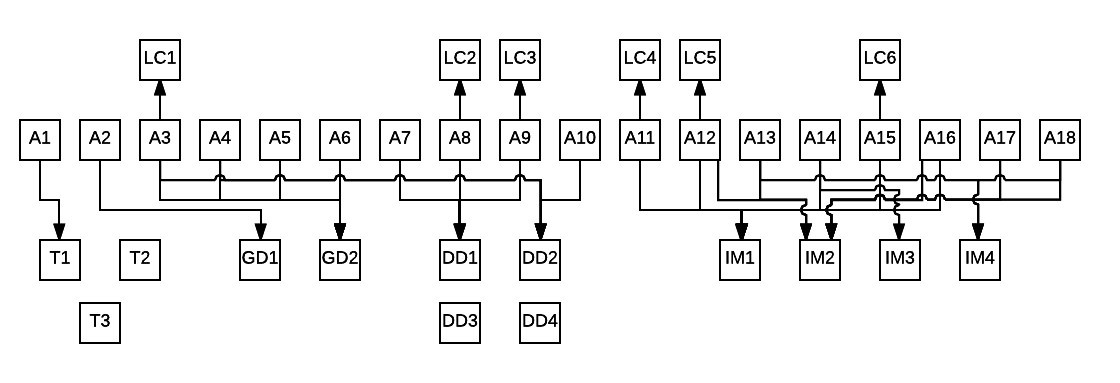
\includegraphics[width=\textwidth]{ATrace.png}
		}
		\caption{\label{Fig_ATrace} Traceability Matrix Showing the Connections Between Items of Different Sections}
	\end{center}
\end{figure}


\begin{figure}[h!]
	\begin{center}
		%\rotatebox{-90}
		{
			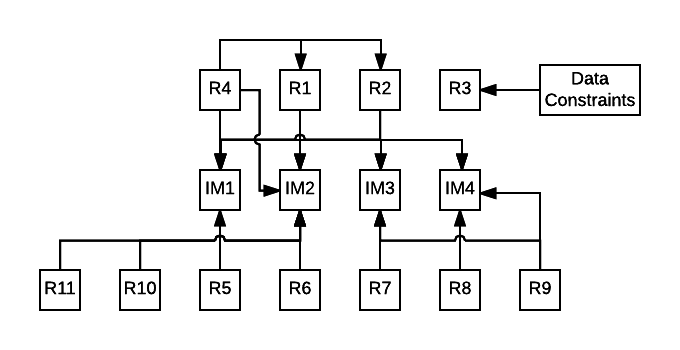
\includegraphics[width=0.7\textwidth]{RTrace.png}
		}
		\caption{\label{Fig_RTrace} Traceability Matrix Showing the Connections Between Requirements, Instance Models, and Data Constraints}
	\end{center}
\end{figure}

\newpage

\bibliographystyle {plain}
\bibliography {PCM_SRS}

\end{document}